\documentclass[a4paper,11pt,twoside]{scrartcl}
\usepackage[T1]{fontenc}
\usepackage{subcaption}
\usepackage[utf8]{inputenc}
\usepackage{ngerman, eucal, mathrsfs, amsfonts, bbm, amsmath, amssymb, stmaryrd,graphicx, array, geometry, color, wrapfig, float, hyperref}
\geometry{left=25mm, right=15mm, bottom=25mm}
\setlength{\parindent}{0em} 
\setlength{\headheight}{0em} 
\title{Machine Learning\\ Blatt 8}
\author{Markus Vieth\and David Klopp\and Christian Stricker}
\date{\today}
\input{../head/lstlisting.tex}
\begin{document}

\newcommand{\cor}[1]{\textcolor{red}{\textit{#1}}}
\maketitle
\cleardoublepage
\pagestyle{myheadings}
\markboth{Markus Vieth,  David Klopp, Christian Stricker}{Markus Vieth, David Klopp, Christian Stricker}

\newpage

\section*{Nr. 3.1}
Design a two-input perceptron that implements the boolean function $A \land \neg B$\\

\subsection*{1. Allgemein:} \[w_0 + w_1 \cdot x_1 + w_2 \cdot x_2\]

\subsection*{2. Bedingungen:}

\[\text{I.}~w_0 - w_1 - w_2 \leq 0 \]
\[\text{II.}~w_0 - w_1 + w_2 \leq 0 \]
\[\text{III.}~w_0 + w_1 - w_2 > 0 \]
\[\text{VI.}~w_0 + w_1 + w_2 \leq 0 \]

\subsection*{3. Rechnung:}

\subsubsection*{1. I + VI}
\[2 \cdot w_0 \leq 0 \Leftrightarrow w_0 \leq 0 \]

\subsubsection*{2.}
\[\text{I.} \Leftrightarrow w_0 \leq w_1 + w_2\]
\[\text{III.} \Leftrightarrow w_0 > -w_1 + w_2\]
\[\Rightarrow -w_1 + w_2 <  w_0 \leq w_1 + w_2\]
\[\Rightarrow -w_1 + w_2 < w_1 + w_2\]
\[ \Leftrightarrow w_1 > 0\]

\subsubsection*{3. Wähle $w_0 = 0$ und $w_1 = 1$}

\[ 0 -1 -w_2 \leq 0\]
\[ -1 \leq w_2\]
\subsubsection*{4. Wähle $w_2 = -1$}

\[\text{I.}~0 - 1 +1 = 0 \leq 0~~~\checkmark \]
\[\text{II.}~0 - 1 - 1 = -2 \leq 0~~~\checkmark \]
\[\text{III.}~0 + 1 +1 = 2 > 0~~~\checkmark \]
\[\text{VI.}~0 + 1 -1 = 0 \leq 0~~~\checkmark \]

\subsubsection*{5. Lösung:}
\[
\overset{\rightarrow}{w} = \begin{pmatrix}
           0 \\
           1 \\
           -1
         \end{pmatrix}
\] 

\pagebreak

\section*{Nr. 3.2}
\begin{figure}[H]
\centering
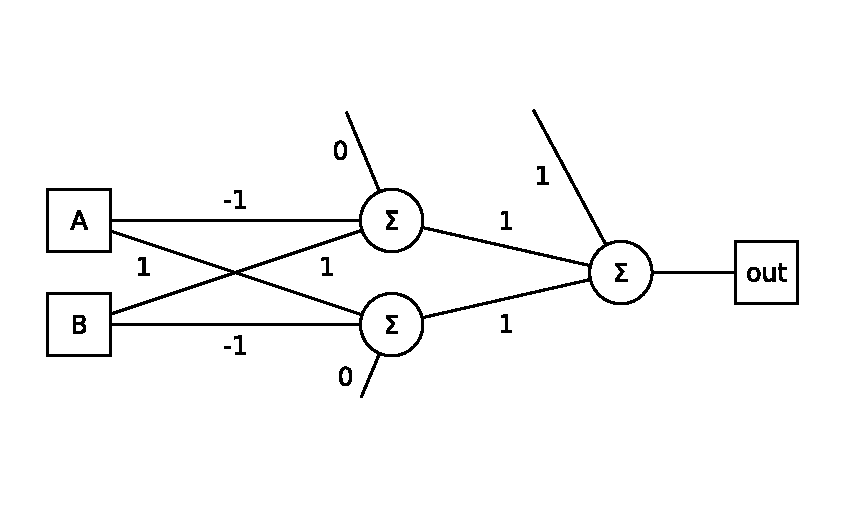
\includegraphics{2Layer}
\caption{Zahlen entsprechen Gewichten, Kanten ins Leere entsprechen $w_0$. Die erste Schicht entspricht der Teilaufgabe 1, zweite Schicht einem Oder $\Rightarrow~~ (A\land\bar{B})\lor(\bar{A}\land B)$}
\label{fig:2Layer}
\end{figure}

\end{document}